% "Your VLA is Secretly kNN" -- CoRL 2026 workshop paper (4-page main text; references and appendix unlimited).
% Build: `make` in this directory. Numbers, tables and figures are generated from the experiment logs by
% ../poster/scripts (KNN_FIG_TARGET=paper).
\documentclass{article}

\usepackage{corl_2026}  % initial (anonymous) submission
\usepackage[utf8]{inputenc}
\usepackage{amsmath,amssymb}
\usepackage{booktabs,tabularx,array}
\usepackage[table]{xcolor}
\usepackage{graphicx}
\usepackage{enumitem}
\DeclareUnicodeCharacter{2212}{\ensuremath{-}}

\definecolor{knn}{HTML}{EB6834}
\definecolor{learned}{HTML}{2A78D6}
\definecolor{tint}{HTML}{F5F6F8}
\newcommand{\knnword}{\textcolor{knn}{\textbf{kNN}}}
\newcommand{\hl}[1]{\textbf{#1}}
% generated by poster/scripts/make_figures.py -- do not edit
\newcommand{\KnnAvg}{91.7}
\newcommand{\KnnPlainResnet}{88.7}
\newcommand{\KnnLearnt}{93.0}
\newcommand{\KnnFullLearnt}{93.0}
\newcommand{\KnnPiZeroBaseLt}{86.9}
\newcommand{\KnnPiZeroLt}{17.9}
\newcommand{\AblNoLang}{64.6}
\newcommand{\AblPixels}{57.2}
\newcommand{\DemosTen}{77.4}
\newcommand{\PlusKnn}{82.4}
\newcommand{\PlusN}{420}
\newcommand{\PlusPerCat}{60}
\newcommand{\PlusXvlaCamera}{7}
\newcommand{\PlusSmolLanguage}{22}
\newcommand{\PlusSmolCtrl}{82}
\newcommand{\PlusFastLanguage}{33}
\newcommand{\PlusFastCtrl}{88}
\newcommand{\PlusPiZeroLanguage}{12}
\newcommand{\PlusPiZeroCtrl}{68}
\newcommand{\KnnDrop}{9.3}
\newcommand{\MinVlaDrop}{12.2}
\newcommand{\MaxVlaDrop}{64.8}
\newcommand{\VlaN}{9}
\newcommand{\KnnRankLibero}{7}
\newcommand{\KnnRankPlus}{3}
\newcommand{\RankN}{10}
\newcommand{\KnnBestPlusSuites}{two}
\newcommand{\FailBase}{8}
\newcommand{\FailMin}{20}
\newcommand{\FailMax}{46}
\newcommand{\LiftMin}{2.4}
\newcommand{\LiftMax}{5.5}
\newcommand{\TaskCorrMedian}{0.74}
\newcommand{\KeyN}{9}
\newcommand{\BeatenClean}{2}
\newcommand{\KeyNPlus}{9}
\newcommand{\BeatenPlus}{4}
\newcommand{\FtN}{8}
\newcommand{\FtUp}{7}
\newcommand{\FtUpMin}{5}
\newcommand{\FtUpMax}{37}
\newcommand{\FtCleanUp}{5}
\newcommand{\SubtractMax}{48}
\newcommand{\LookupPi}{0.90}
\newcommand{\LookupHuman}{0.78}
\newcommand{\HeadPlusPi}{0.85}
\newcommand{\HeadPlusJepa}{0.68}
\newcommand{\HeadPlusSmol}{0.08}
\newcommand{\HeadPlusFast}{-0.01}
\newcommand{\NmOtherMin}{0.76}
\newcommand{\NmOtherMax}{0.88}
\newcommand{\NmFairRho}{0.61}
\newcommand{\NmFairR}{0.78}
\newcommand{\NmFairN}{12}
\newcommand{\NmPiZeroLibero}{0.55}
\newcommand{\MapN}{4,150}
\newcommand{\MapGoalResnet}{79}
\newcommand{\MapGoalPromptMin}{96}
\newcommand{\MapGoalCausalMin}{76}
\newcommand{\MapGoalCausalMax}{82}
\newcommand{\MapPhaseN}{8}
\newcommand{\MapPhaseDown}{7}
\newcommand{\MapPhaseEvoBefore}{0.031}
\newcommand{\MapPhaseEvoAfter}{0.022}
\newcommand{\MapPhasePiZeroBefore}{0.028}
\newcommand{\MapPhasePiZeroAfter}{0.052}
\newcommand{\MapGoalPiZeroAfter}{100}
\newcommand{\MapSuiteResnet}{85}
\newcommand{\MapSuiteBeforeMin}{40}
\newcommand{\MapSuiteBeforeMax}{84}
\newcommand{\MapSuiteAfterMin}{1}
\newcommand{\MapSuiteAfterMax}{43}
\newcommand{\MapSuiteDown}{8}
\newcommand{\OptunaN}{24}
\newcommand{\OptunaAll}{193}
\newcommand{\OptunaK}{57}
\newcommand{\OptunaOne}{25}
\newcommand{\RetryBase}{80.8}
\newcommand{\RetryMin}{78.5}
\newcommand{\RetryMax}{81.3}


\setlist{leftmargin=1.3em, itemsep=0.15em, topsep=0.3em, parsep=0pt}

\title{Your VLA is Secretly kNN: A Training-Free Probe for\\Task Difficulty, Backbones and Action Heads}

\author{Anonymous Authors}

\begin{document}
\maketitle

\begin{abstract}
Vision-language-action (VLA) models now exceed 95\% success on dense simulation benchmarks such as LIBERO, but it is
unclear what such numbers measure. We use a training-free $k$-nearest-neighbour lookup over the demonstrations, not as
a controller but as a probe. On LIBERO it solves \KnnAvg\% of the official evaluation without training; nine public
VLAs fail on the same tasks, and a lookup predicts their action chunks as well as it predicts a held-out human
demonstration. Under the perturbations of LIBERO-plus the lookup degrades least of all the policies we test, while VLAs
lose up to \MaxVlaDrop\ points. Keying the same lookup on a VLA's own vision-language model separates the backbone from
the action head, before and after fine-tuning: fine-tuning mostly makes the backbone a more robust key, it can also
break it, and some action heads are worse than a lookup on their own backbone. A neighbour metric computed offline
tracks backbone quality without rollouts. The probe is a LeRobot policy plugin, so any benchmark LeRobot runs can
run the test.
\end{abstract}

\keywords{Vision-language-action models, evaluation, nearest neighbours}

%===============================================================================
\section{Introduction}

Vision-language-action models are fine-tuned on a few dozen demonstrations per task and evaluated in simulation, where
the strongest now succeed in 97\% of LIBERO episodes~\citep{liu2023libero}. Such a number says little by itself: the
test scenes are close to the demonstrations, so a policy can succeed by recalling them. Nor does it say which part of
a VLA works, the pretrained vision-language backbone or the action head trained on top of it.

We propose a simple instrument for both questions: a $k$-nearest-neighbour (kNN) lookup over the demonstration frames,
which executes the actions that followed the frames closest to the current observation. It is \emph{not} a proposal
for robot control: a lookup cannot extrapolate beyond its memory. That is what makes it useful as a probe. It answers
three questions without training anything:
\begin{enumerate}
  \item \textbf{How hard is the task?} What a lookup over generic image features already solves is retrieval, not
        generalisation (\S\ref{sec:task}).
  \item \textbf{How good is the backbone, and what did fine-tuning do to it?} The same lookup keyed on a VLA's own
        vision-language model (VLM), before and after fine-tuning, or offline, without rollouts (\S\ref{sec:inside}).
  \item \textbf{How good is the action head?} Its margin over a lookup on its own backbone (\S\ref{sec:inside}).
\end{enumerate}
We implement the probe as a policy plugin for LeRobot~\citep{cadene2024lerobot}: it is fitted from any LeRobot
dataset with one command and evaluated with the standard \texttt{lerobot-eval}, so the test runs on any benchmark that
LeRobot supports, and any VLA in LeRobot can serve as its key.

We apply the probe to nine public LIBERO fine-tunes~\citep{pi2025pi05,fang2026molmoact2,sun2026vlajepa,lin2026evo1,
nvidia2025gr00t,zheng2026xvla,pertsch2025fast,shukor2025smolvla,black2024pi0} on LIBERO and on the perturbed scenes of
LIBERO-plus~\citep{fei2025liberoplus}.

\textbf{Related work.} Retrieval has been used as a policy~\citep{pari2022vinn,he2025alt,mishra2026cfdp}, to select
training data~\citep{du2023behaviorretrieval,memmel2025strap}, and as context for agents and
VLAs~\citep{sridhar2025regent,sridhar2025ricl}, where a plain nearest-neighbour replay already rivals generalist
agents~\citep{sridhar2025regent}; \citet{he2025alt} argue that diffusion policies memorise an action lookup table.
Perturbation benchmarks show that VLAs memorise action sequences and layouts~\citep{fei2025liberoplus,zhou2025liberopro,
xu2025affordance}, interpretability work finds episode-specific memorisation features~\citep{swann2026sae} and separate
roles for VLM and action pathways~\citep{grant2026features}, and VLA fine-tuning is known to erode the VLM's
vision-language skills~\citep{driess2025insulating,grover2025preserving,zhang2026vlm4vla}. We turn retrieval into an
instrument: it measures how much of a benchmark is retrieval, scores a VLA's backbone \emph{as an action-relevant key}
by closed-loop success, before and after fine-tuning, and measures what its action head adds.

%===============================================================================
\section{A kNN probe}
\label{sec:method}

\textbf{The policy.} The memory holds every second frame of the 1{,}693 LIBERO demonstrations (137k keys), each with the
chunk of actions that followed. ``Training'' is embedding them. At test time the policy embeds the observation $o$ with
$\phi$ and executes
\begin{equation}
  \pi(o)\;=\sum_{i\,\in\,\mathcal N_k(o)} w_i\, a_{t_i:t_i+H}, \qquad w_i \propto e^{-d(o,\,o_i)/\tau},
\end{equation}
over the $k$ nearest demonstration frames $o_i$, at most one per demonstration. The distance $d$ adds image distances
(per camera), state, prompt (CLIP~\citep{radford2021clip}), time-in-episode and history terms, each scaled by its median
within the task. Two extras make the average safe: \emph{mode seeking} down-weights neighbours whose chunks disagree
with the dominant one instead of averaging them into an action no demonstrator took, and \emph{temporal ensembling}
blends overlapping chunks~\citep{zhao2023act}. Every executed action is therefore a convex combination of demonstrated
actions. An optional \emph{retry} rewinds and retrieves again when the scene looks unlike any demonstration; it did not
help and is off. Hyper-parameters were tuned with Optuna~\citep{akiba2019optuna} (Appendix~\ref{app:knn}). With a frozen
ImageNet ResNet-18~\citep{he2016resnet} key (layer 3, $4\times4$ grid per camera), this \emph{full method} needs no
training; the \emph{plain lookup} drops every extra.

\textbf{VLM keys.} Any VLA's vision-language model can be the key $\phi$: the hidden states of one layer over each
camera's image tokens, standardised per dimension (VLM residual streams are dominated by a few massive
activations~\citep{sun2024massive}) and pooled to a $2\times2$ grid. The layer is chosen once per family by an offline
pilot (held-out action $R^2$) and kept for the checkpoints before and after LIBERO fine-tuning.

\textbf{Offline score.} A lookup only uses the nearest neighbours, so we score a key by its local action consistency,
LAC@8\,=\,1\,$-$\,the action distance from a held-out frame to its 8 nearest frames of other demonstrations, divided by
the distance to a random frame of the same task.

%===============================================================================
\section{Setup}

\textbf{LIBERO}~\citep{liu2023libero}: 4 suites $\times$ 10 tasks, $\sim$42 demonstrations per task. Every policy runs the
official protocol, 50 episodes per task (2{,}000; the full kNN method with \texttt{lerobot-eval}, the others in our
evaluation harness on the same initial states). \textbf{LIBERO-plus}~\citep{fei2025liberoplus}: the same tasks under seven
perturbations (camera, robot initial state, language, light, background, sensor noise, layout); a fixed sample of
\PlusN\ of its 10{,}030 variants (\PlusPerCat\ per perturbation), the same for every policy, never trained on.
\textbf{VLAs}: nine public LIBERO checkpoints from the LeRobot Hub~\citep{cadene2024lerobot}, evaluated as released
(Appendix~\ref{app:vlas}). Nothing is trained except the optional learnt key of \S\ref{sec:lac}.

%===============================================================================
\section{How hard is the task?}
\label{sec:task}

\begin{table}[t]
  \centering\scriptsize\setlength{\tabcolsep}{2.5pt}
  \begin{tabularx}{\linewidth}{@{}l*{5}{>{\raggedleft\arraybackslash}X}@{\hspace{3mm}}*{5}{>{\raggedleft\arraybackslash}X}@{\hspace{3mm}}>{\raggedleft\arraybackslash}X@{}}
\toprule
 & \multicolumn{5}{c}{LIBERO} & \multicolumn{5}{c}{LIBERO-plus} & \\
\cmidrule(lr){2-6}\cmidrule(lr){7-11}
 & avg & Spat & Obj & Goal & Long & avg & Spat & Obj & Goal & Long & drop \\
\midrule
$\pi_{0.5}$ & \textbf{97.7} & 97 & 100 & \textbf{98} & \textbf{96} & \textbf{85.5} & \textbf{90} & 84 & 83 & \textbf{85} & −12.2 \\
MolmoAct2 & 97.5 & \textbf{97} & 99 & 98 & 96 & 82.6 & 90 & 82 & 76 & 83 & −14.9 \\
\rowcolor{tint}\knnword{}, full method & 91.7 & 88 & 100 & 98 & 81 & 82.4 & 79 & \textbf{86} & \textbf{87} & 78 & \textbf{−9.3} \\
\rowcolor{tint}\knnword{}, + learnt key & 93.0 & 91 & 100 & 97 & 85 & 81.7 & 88 & 84 & 81 & 74 & −11.3 \\
GR00T N1.7 & 94.8 & 96 & 98 & 95 & 91 & 80.2 & 90 & 74 & 79 & 78 & −14.6 \\
\rowcolor{tint}\knnword{}, plain & 88.7 & 90 & 95 & 95 & 74 & 75.5 & 77 & 82 & 79 & 64 & −13.2 \\
VLA-JEPA & 97.2 & 95 & \textbf{100} & 97 & 96 & 74.0 & 81 & 70 & 77 & 68 & −23.1 \\
Evo-1 & 95.4 & 92 & 99 & 97 & 94 & 71.4 & 74 & 73 & 70 & 69 & −24.0 \\
X-VLA & 94.5 & 95 & 99 & 93 & 92 & 64.5 & 71 & 65 & 65 & 57 & −30.0 \\
$\pi_0$ & 71.9 & 70 & 86 & 86 & 45 & 42.9 & 54 & 42 & 47 & 29 & −29.0 \\
SmolVLA & 82.2 & 79 & 92 & 88 & 70 & 27.9 & 30 & 50 & 11 & 20 & −54.3 \\
$\pi_0$-FAST & 90.5 & 90 & 94 & 91 & 87 & 25.7 & 39 & 34 & 16 & 13 & −64.8 \\
\bottomrule
\end{tabularx}

  \caption{Success (\%) on LIBERO (official protocol, 2{,}000 episodes) and on the same LIBERO-plus variants, ordered by
  LIBERO-plus. The kNN rows are training-free except the learnt key. Bold: best per column.}
  \label{tab:results}
\end{table}

Table~\ref{tab:results} places the lookup among the VLAs. \textbf{A training-free lookup is competitive}: \KnnAvg\% on
LIBERO, rank \KnnRankLibero\ of \RankN. \textbf{Under perturbation it degrades least}: \KnnDrop\ points, against
\MinVlaDrop\ for the most robust VLA and up to \MaxVlaDrop; it ranks \KnnRankPlus\ and is the best policy on
\KnnBestPlusSuites\ suites. Part of this is a favourable benchmark: LIBERO-plus scenes need the same actions as the clean
demonstrations, so the answer is in memory whenever the key ignores the perturbation.

\textbf{VLAs fail where the lookup fails.} When a VLA fails a LIBERO episode, the lookup fails the same episode in
\FailMin--\FailMax\% of cases, against \FailBase\% overall (\LiftMin--\LiftMax$\times$ chance), and per-task success
correlates with the lookup's (median $r$\,=\,\TaskCorrMedian; Appendix~\ref{app:more}). The weak VLAs key on the
wording: reworded instructions over the original scenes drop SmolVLA, $\pi_0$-FAST and $\pi_0$ to \PlusSmolLanguage,
\PlusFastLanguage\ and \PlusPiZeroLanguage\% (original wording: \PlusSmolCtrl, \PlusFastCtrl, \PlusPiZeroCtrl\%).

%===============================================================================
\section{Inside the VLAs}
\label{sec:inside}

\begin{figure}[t]
  \centering
  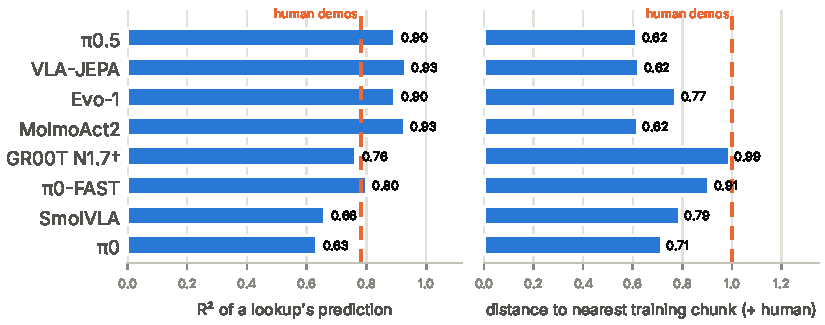
\includegraphics[width=\linewidth]{figures/vla_lookup.pdf}
  \caption{Clean LIBERO rollouts of each VLA. Left: $R^2$ of a lookup over the demonstrations (ResNet-18 key, $k=8$)
  predicting the VLA's action chunk at the same state; dashed: the same for held-out human demonstrations. Right: the
  chunk's distance to the nearest training chunk, relative to a held-out human demonstration's. $^\dagger$Spatial suite.
  X-VLA predicts absolute poses and is left out.}
  \label{fig:lookup}
\end{figure}

\textbf{VLAs act like a lookup.} At the states a VLA visits, a lookup over the demonstrations predicts its action chunk
as well as it predicts a held-out human demonstration, or better ($R^2$\,=\,\LookupPi\ for $\pi_{0.5}$, \LookupHuman\
for humans; Fig.~\ref{fig:lookup}), and the VLA's chunks are closer to a training chunk than a new human demonstration
is: they are not new. Off the demonstrations, on recorded LIBERO-plus rollouts, the robust VLAs stay lookup-like in their
own key space ($R^2$\,=\,\HeadPlusPi\ for $\pi_{0.5}$, \HeadPlusJepa\ for VLA-JEPA), the collapsing ones do not
(\HeadPlusSmol\ for SmolVLA, \HeadPlusFast\ for $\pi_0$-FAST).

\begin{table}[t]
  \centering\footnotesize\setlength{\tabcolsep}{3pt}
  \begin{tabularx}{\linewidth}{@{}l*{6}{>{\raggedleft\arraybackslash}X}@{}}
\toprule
 & \multicolumn{3}{c}{LIBERO} & \multicolumn{3}{c}{LIBERO-plus} \\
\cmidrule(lr){2-4}\cmidrule(lr){5-7}
 & \knnword{} before & \knnword{} after & VLA & \knnword{} before & \knnword{} after & VLA \\
\midrule
$\pi_{0.5}$ & 85.4 & 81.8 & \textcolor{learned}{97.7} & 60.5 & 65.7 & \textcolor{learned}{85.5} \\
MolmoAct2 & 78.6 & 91.3 & \textcolor{learned}{97.5} & 52.6 & 81.0 & \textcolor{learned}{82.6} \\
GR00T N1.7* & 87.5 & 87.5 & \textcolor{learned}{94.8} & 66.4 & 66.4 & \textcolor{learned}{80.2} \\
VLA-JEPA & 84.0 & 83.0 & \textcolor{learned}{97.2} & 49.3 & 65.7 & \textcolor{learned}{74.0} \\
Evo-1 & 62.1 & 87.1 & \textcolor{learned}{95.4} & 35.5 & \textcolor{knn}{\textbf{72.6}} & \textcolor{learned}{71.4} \\
X-VLA & 83.3 & 88.5 & \textcolor{learned}{94.5} & 62.4 & \textcolor{knn}{\textbf{78.1}} & \textcolor{learned}{64.5} \\
$\pi_0$ & 86.9 & 17.9 & \textcolor{learned}{71.9} & 56.7 & 2.4 & \textcolor{learned}{42.9} \\
SmolVLA & 76.3 & \textcolor{knn}{\textbf{86.5}} & \textcolor{learned}{82.2} & 45.0 & \textcolor{knn}{\textbf{69.3}} & \textcolor{learned}{27.9} \\
$\pi_0$-FAST & 86.6 & \textcolor{knn}{\textbf{95.0}} & \textcolor{learned}{90.5} & 58.3 & \textcolor{knn}{\textbf{74.0}} & \textcolor{learned}{25.7} \\
\bottomrule
\end{tabularx}

  \caption{A plain lookup keyed on each VLA's own VLM before and after its LIBERO fine-tuning, and the VLA itself
  (success, \%). Orange: the lookup on the fine-tuned VLM beats the VLA. $^{*}$GR00T froze its VLM, so before
  $=$ after.}
  \label{tab:backbones}
\end{table}

\textbf{Backbone and action head.} A lookup keyed on a VLA's own VLM scores its backbone; the VLA's excess over it is
its action head's (Table~\ref{tab:backbones}). \emph{Some action heads subtract}: \BeatenClean\ of \KeyN\ VLAs score below
a lookup on their own fine-tuned VLM on LIBERO, \BeatenPlus\ of \KeyNPlus\ under perturbation, by up to \SubtractMax\
points. GR00T froze its VLM during fine-tuning, so everything it learned on LIBERO is in its action head.

\begin{figure}[t]
  \centering
  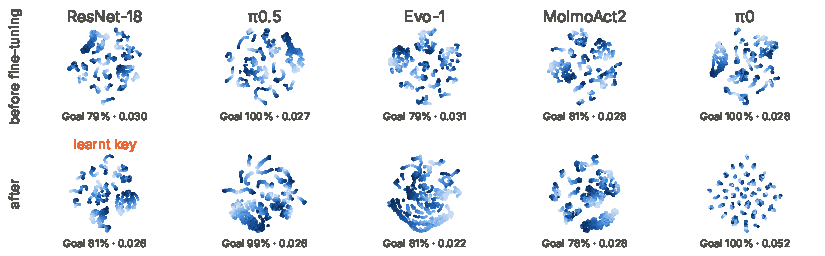
\includegraphics[width=\linewidth]{figures/embedding_pairs.pdf}
  \caption{t-SNE of the lookup keys of the same \MapN\ demonstration frames, coloured by progress through the episode
  (light: start, dark: end), before (top) and after (bottom) LIBERO fine-tuning. Below each map: same-task nearest neighbours from other
  demonstrations on LIBERO-Goal (one scene, ten instructions) and the median progress gap to them.}
  \label{fig:maps}
\end{figure}

\textbf{What fine-tuning does to the backbone.} It mostly makes the VLM a more robust key: +\FtUpMin\ to +\FtUpMax\
points on LIBERO-plus for \FtUp\ of \FtN\ VLAs, while clean success improves for only \FtCleanUp. Maps of the keys show
what changes (Fig.~\ref{fig:maps}, Appendix~\ref{app:maps}): the scene stops dominating them, and they track the phase of
the task (the progress gap shrinks for \MapPhaseDown\ of \MapPhaseN\ VLMs). Fine-tuning can also break the backbone:
$\pi_0$'s key still tells the tasks apart but loses the phase (\MapPhasePiZeroBefore\,$\to$\,\MapPhasePiZeroAfter), and
its lookup collapses (\KnnPiZeroBaseLt\,$\to$\,\KnnPiZeroLt\%).

\textbf{Scoring a backbone without rollouts.}
\label{sec:lac}
LAC tracks the closed-loop success of a lookup with each key (Pearson $r$\,=\,\NmFairR, Spearman
$\rho$\,=\,\NmFairRho\ over the \NmFairN\ keys that never saw these demonstrations; Appendix~\ref{app:more}) and flags a
broken backbone: $\pi_0$'s fine-tuned key has LAC \NmPiZeroLibero, against \NmOtherMin--\NmOtherMax\ for every other key. Fine-tuned VLMs score high on their own training demonstrations, so LAC on
them flags memorisation. As a loss (one linear map per ResNet grid cell) it lifts the plain lookup
\KnnPlainResnet\,$\to$\,\KnnLearnt\% and the full method to \KnnFullLearnt\%.

%===============================================================================
\section{Limitations and conclusion}

LIBERO has dense demonstrations and test scenes close to them, the regime where retrieval works; our LIBERO-plus numbers
come from a 420-variant sample (about $\pm$3.5 points overall), and its perturbed scenes keep the demonstrated actions
valid. A lookup cannot extrapolate beyond its memory: we propose it not for robot control but as a cheap, training-free
test to report next to every VLA result on a dense-demonstration benchmark (how much of it is retrieval, how good the
backbone is and what fine-tuning did to it, what the action head adds), on any benchmark LeRobot supports.

\clearpage
\acknowledgments{Withheld for review.}
\bibliography{refs}

%===============================================================================
\clearpage
\appendix

\section{The kNN policy: tuning and ablations}
\label{app:knn}

\begin{figure}[h]
  \centering
  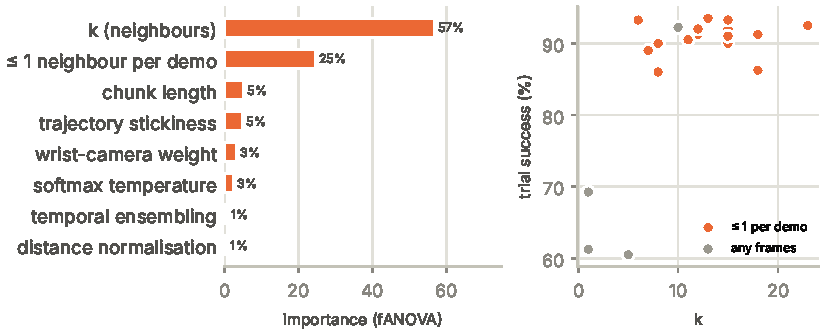
\includegraphics[width=\linewidth]{figures/optuna.pdf}
  \caption{Hyper-parameter search (Optuna, \OptunaN\ trials of 400 episodes in the final study, \OptunaAll\ over all
  studies, on initial states 40--49 and 0--19). Left: fANOVA importance~\citep{hutter2014fanova}. Right: every trial's
  success against $k$. LIBERO has no held-out split, so the official evaluation includes these states, as for every
  LIBERO result.}
\end{figure}

\begin{table}[h]
  \centering\footnotesize\setlength{\tabcolsep}{4pt}
  \begin{tabularx}{\linewidth}{@{}X*{6}{r}@{}}
\toprule
Change to the full method & avg & Spatial & Object & Goal & Long & $\Delta$ \\
\midrule
none (full method, \texttt{lerobot-eval}) & 91.7 & 88.0 & 99.8 & 97.6 & 81.4 & \\
prompt ignored & 64.6 & 77.6 & 99.6 & 8.8 & 72.4 & −27.1 \\
raw 16$\times$16 pixels & 57.1 & 79.0 & 0.0 & 91.0 & 58.6 & −34.6 \\
10\% of demos & 77.4 & 83.8 & 87.0 & 90.2 & 48.6 & −14.3 \\
25\% of demos & 82.6 & 83.6 & 97.8 & 92.6 & 56.4 & −9.1 \\
50\% of demos & 88.5 & 86.4 & 99.6 & 95.4 & 72.6 & −3.2 \\
k = 1 (replay nearest demo) & 78.6 & 77.2 & 90.6 & 86.2 & 60.4 & −13.1 \\
DINOv2-S instead of ResNet-18 & 83.4 & 79.8 & 97.6 & 95.0 & 61.0 & −8.3 \\
agent-view camera only & 82.0 & 78.0 & 92.8 & 93.6 & 63.8 & −9.7 \\
wrist camera only & 87.5 & 87.0 & 98.8 & 92.8 & 71.2 & −4.2 \\
plain weighted mean & 90.7 & 88.4 & 100.0 & 96.6 & 77.8 & −1.0 \\
no temporal ensembling & 91.1 & 92.0 & 98.0 & 94.2 & 80.2 & −0.6 \\
no history matching & 91.5 & 89.6 & 98.8 & 97.6 & 79.8 & −0.2 \\
no proprioceptive state & 91.3 & 87.6 & 99.6 & 96.8 & 81.4 & −0.4 \\
no time-step feature & 91.3 & 88.2 & 99.8 & 97.4 & 79.8 & −0.4 \\
hard task filter & 91.9 & 88.4 & 100.0 & 97.4 & 81.8 & +0.2 \\
\midrule
$k$ = 2 (13 in the full method) & 85.2 & 83.8 & 94.6 & 92.2 & 70.2 & −6.5 \\
$k$ = 4 (13 in the full method) & 89.3 & 86.2 & 98.8 & 93.8 & 78.6 & −2.4 \\
$k$ = 8 (13 in the full method) & 89.8 & 85.4 & 99.6 & 96.6 & 77.6 & −1.9 \\
$k$ = 24 (13 in the full method) & 92.7 & 89.2 & 99.8 & 97.2 & 84.4 & +1.0 \\
$k$ = 32 (13 in the full method) & 91.7 & 88.8 & 99.8 & 97.4 & 80.8 & +0.0 \\
\bottomrule
\end{tabularx}

  \caption{One change to the full method at a time, official protocol (2{,}000 episodes). $\Delta$: against the full
  method. $k$\,=\,24 scores slightly above the tuned $k$\,=\,13, within the $\pm$1.2-point 95\% interval of 2{,}000
  episodes. Raw pixels fail all of LIBERO-Object: at $16\times16$ its ten tasks share a scene of small objects.}
\end{table}

\section{Evaluated VLAs}
\label{app:vlas}

All checkpoints are public and evaluated as released, at their LeRobot settings: $\pi_{0.5}$, $\pi_0$ and
$\pi_0$-FAST (LeRobot LIBERO fine-tunes), SmolVLA, X-VLA (absolute end-effector control and its own observation
convention), VLA-JEPA (7 actions per re-plan), Evo-1 (14 actions per re-plan; 256\,px renders on both benchmarks, as
LIBERO-plus noise assumes them), MolmoAct2 (continuous actions), GR00T N1.7 (one checkpoint per suite, 8 of 16
actions per re-plan). Every checkpoint first passes an offline check: on demonstration frames its predicted motion must
be closer to the demonstrated one than half the error of a shuffled pairing.

\section{More results}
\label{app:more}

\begin{figure}[h]
  \centering
  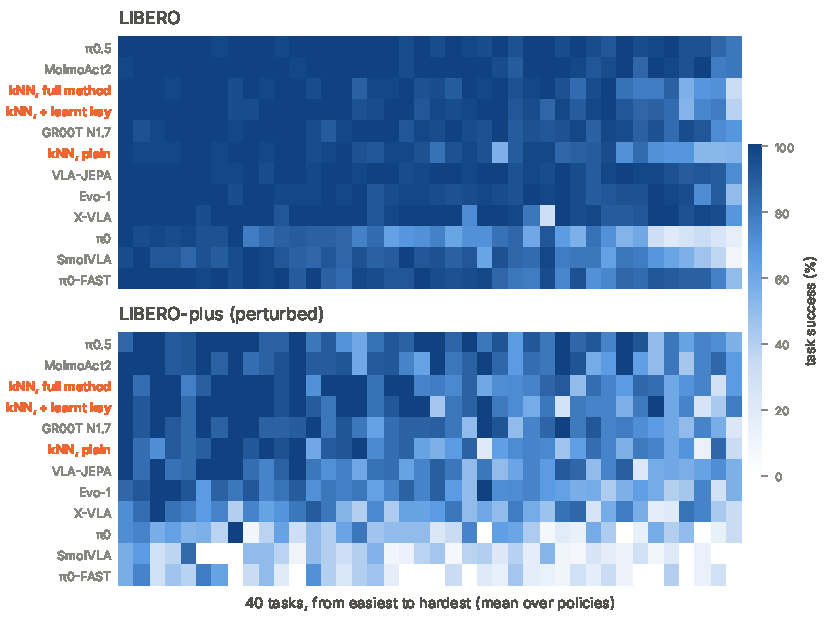
\includegraphics[width=\linewidth]{figures/task_map.pdf}
  \caption{Success of every policy on each of the 40 tasks, tasks sorted from easiest to hardest (mean over policies).}
\end{figure}

\begin{figure}[h]
  \centering
  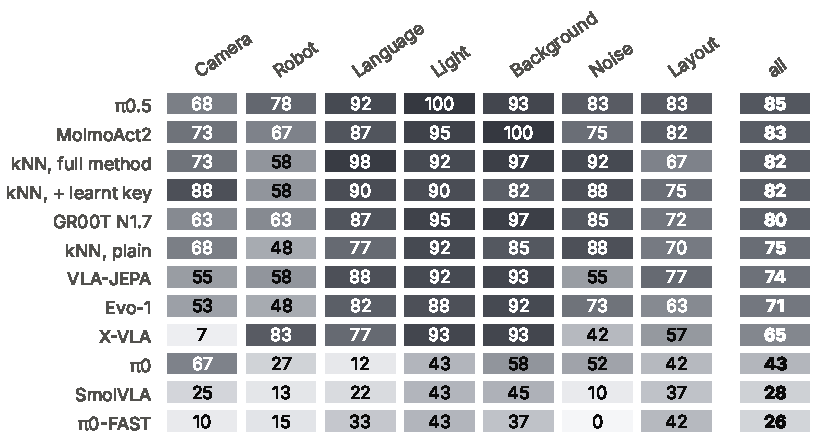
\includegraphics[width=\linewidth]{figures/libero_plus.pdf}
  \caption{LIBERO-plus success (\%) per perturbation, same variants for every policy.}
\end{figure}

\begin{figure}[h]
  \centering
  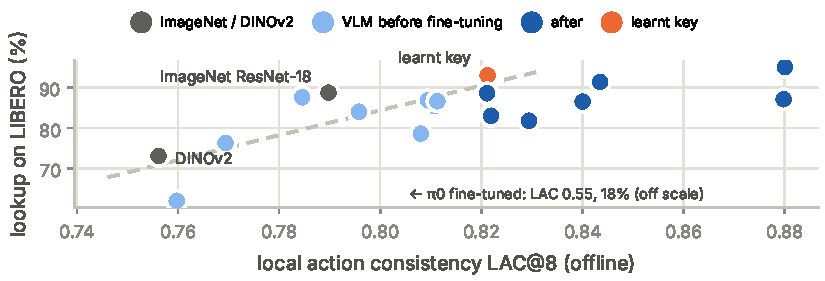
\includegraphics[width=\linewidth]{figures/neighbors.pdf}
  \caption{Local action consistency of a key (offline, held-out queries) against the LIBERO success of a plain lookup
  with that key; one point per backbone key, before and after LIBERO fine-tuning.}
\end{figure}

\clearpage
\section{Embedding maps}
\label{app:maps}

Every key of Table~\ref{tab:backbones}, plus the generic keys, on the same \MapN\ demonstration frames (6 random
demonstrations per task, every 10th frame). Each key is computed as the plain lookup computes it: standardised with
memory statistics, unit-normalised per camera, cameras concatenated. Fig.~\ref{fig:maps-tsne}: t-SNE (perplexity 30, on
the first 50 principal components), coloured by progress through the episode. Fig.~\ref{fig:maps-pca}: the first two
principal components, coloured by suite. Before fine-tuning the suites, i.e.\ the scenes, dominate every key (the suite
explains \MapSuiteBeforeMin--\MapSuiteBeforeMax\% of the variance of the two components; ImageNet ResNet-18:
\MapSuiteResnet\%); after it far less (\MapSuiteAfterMin--\MapSuiteAfterMax\%, lower for \MapSuiteDown\ of
\MapPhaseN\ VLMs), consistent with the fine-tuned keys' robustness to scene perturbations. Only keys whose image tokens
attend to the instruction, under the bidirectional prefix attention of PaliGemma ($\pi_0$, $\pi_{0.5}$, $\pi_0$-FAST)
and of Florence-2's encoder (X-VLA), tell LIBERO-Goal's ten tasks apart: \MapGoalPromptMin--100\% same-task neighbours,
against \MapGoalCausalMin--\MapGoalCausalMax\% for the VLMs with causal attention, whose image tokens precede the
instruction, and \MapGoalResnet\% for ResNet-18.

\begin{figure}[p]
  \centering
  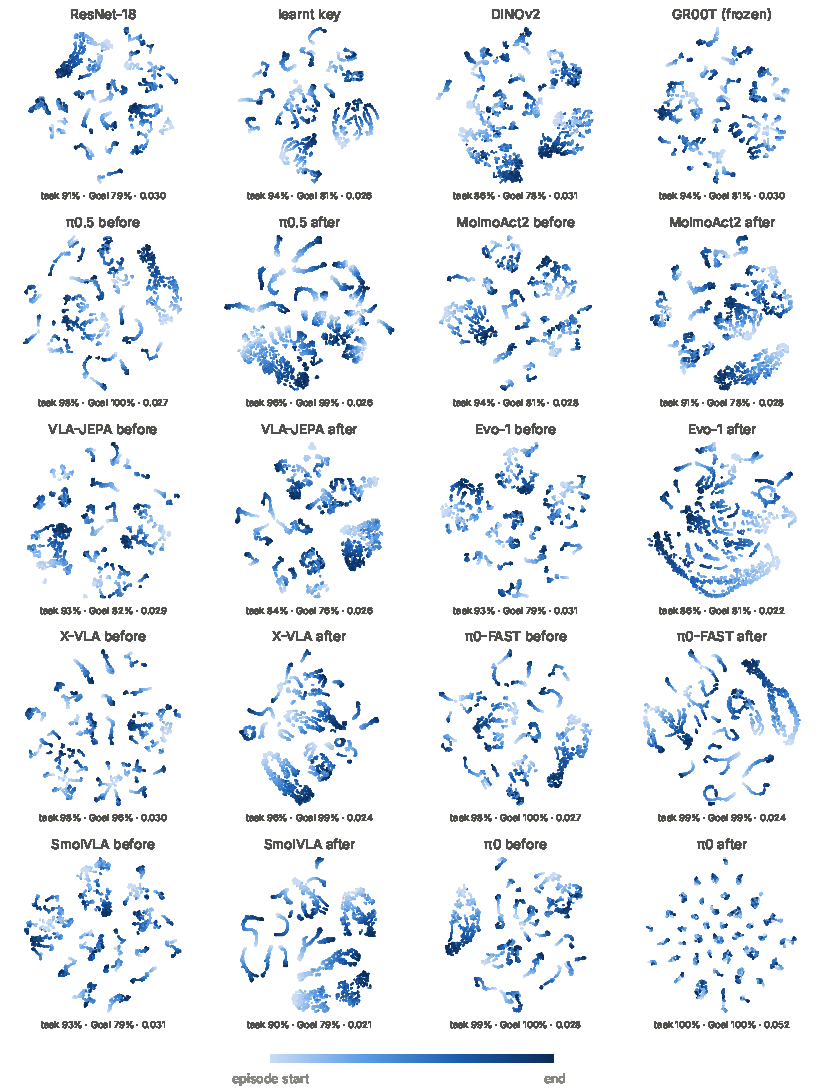
\includegraphics[width=\linewidth]{figures/embedding_tsne_progress.pdf}
  \caption{t-SNE of every key, coloured by progress through the episode. Below each map: same-task nearest neighbours
  from other demonstrations (all tasks; LIBERO-Goal) and the median progress gap to the nearest frame of another
  demonstration of the same task. GR00T froze its VLM, so its key is the same before and after fine-tuning.}
  \label{fig:maps-tsne}
\end{figure}

\begin{figure}[p]
  \centering
  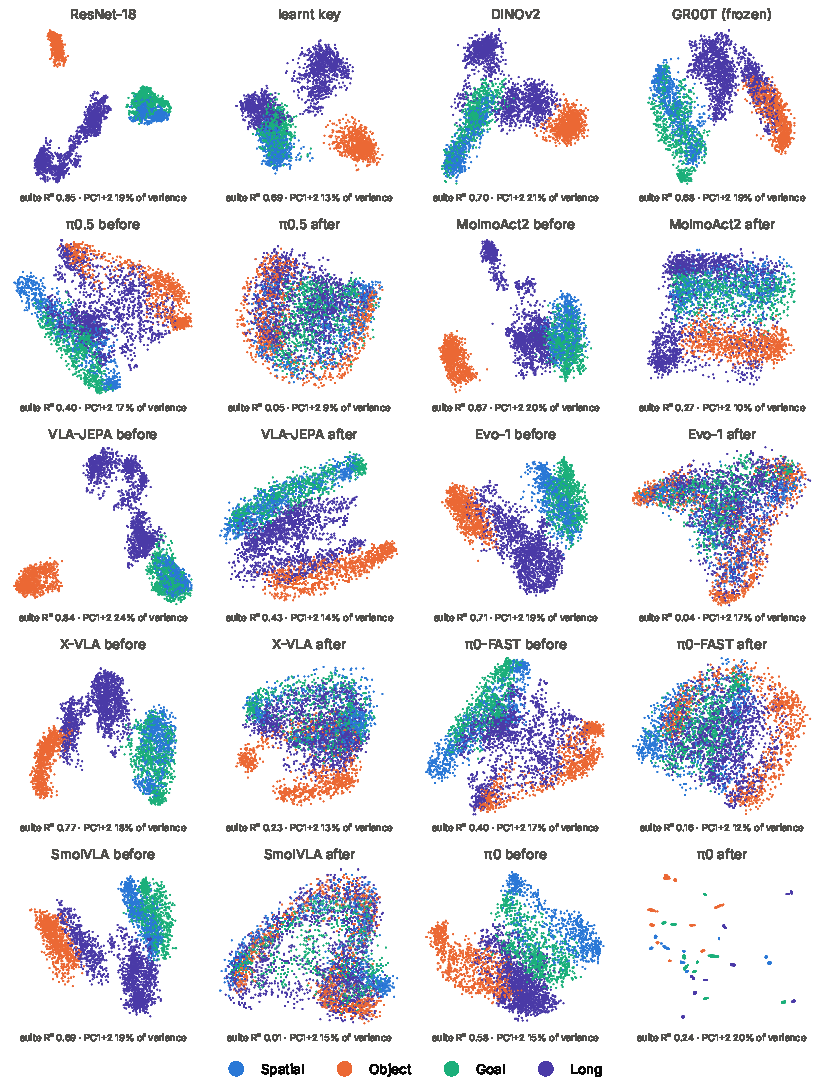
\includegraphics[width=\linewidth]{figures/embedding_pca_suite.pdf}
  \caption{The first two principal components of every key, coloured by suite. Below each map: the share of their
  variance the suite explains, and the share of the key's variance they explain.}
  \label{fig:maps-pca}
\end{figure}

\end{document}
